\section{Approach}\label{s:approach}

In order to honor LC reservations while still running BEs opportunistically, our
approach is to enforce the isolation between them by using priority scheduling.

We show that doing so solves the enforcement problem that weights has, as well
as its dependence on hardware ticks (\autoref{ss:approach:solves-problems}).
Linux has priority scheduling for real time applications, which we show is able
to isolate well between workloads of different priotiries
(\autoref{ss:approach:linux-classes-isolate}), but is not a good fit for
microservice workloads (\autoref{ss:approach:linux-classes-bad-fit}).

\subsection{Priority scheduling solves the problems}\label{ss:approach:solves-problems}

Enforcing isolation of two priorities is simpler and requires fewer cross-core
checks than enforcing a weight split. 

It is simpler because priorities are: a core does not need to do complex
accounting to figure out whether it is a low-weight processes turn to run, it
just needs to know the set of runnable priorities. Enforcing the isolation
between them equivalent to choosing only from the highest priority.

Isolating priorities also requires fewer cross-core checks, because they only
need to happen on \textit{class boundary crossings}: on \exit{}, when a core
switches to running lower class processes after having previously been running
high class, and on \entry{}, when a core enqueues a higher class process. These
checks ensure that if a core is currently running a BE thread $t$, the scheduler
knows that there are no queued and waiting LC threads anywhere: If there were
ones before it started running $t$, the \exit{} check would have stolen it, and
if a new LC thread wakes up while $t$ is running, the \entry{} check ensures
that the core where it wakes up will interrupt $t$.

Strict priorities being enforced at class boundary crossings rather than ticks
also means that the fidelity of the isolation is now dependent on how quickly
the handler for process wakeup or dequeue runs, not on the length of a
scheduling tick. The kernel already runs handlers in the wakeup and exit paths,
and can choose to reschedule or steal work from other cores. 


\subsection{Linux scheduling classes isolate
well}\label{ss:approach:linux-classes-isolate}

Linux already has multiple scheduling classes that are accessible to users,
which are (in descending order of priority): \deadlineclass{}, \rtclass{}, and
\normalclass{}. Generally speaking most load is expected to fall into the
\normalclass{} scheduling class (hence the name). It is the default scheduling
class, and it is only within the \normalclass{} scheduling class that the
\cgroups{} cpu.weight interface is relevant.

Each scheduling class exists completely separately: classes maintain their own
runqueues and per-entity state; implement their own scheduling algorithms to
choose from the entities on their runqueue; and balance the load across
runqueues on different cores. 

Linux isolates strictly between different scheduling classes: it only schedules
a lower scheduling class if the higher scheduling classes found nothing to run,
and each scheduling class tries to steal work from other cores before returning
that it has nothing to run.

\begin{figure}[t]
    \centering
    \begin{subfigure}[t]{\columnwidth}
        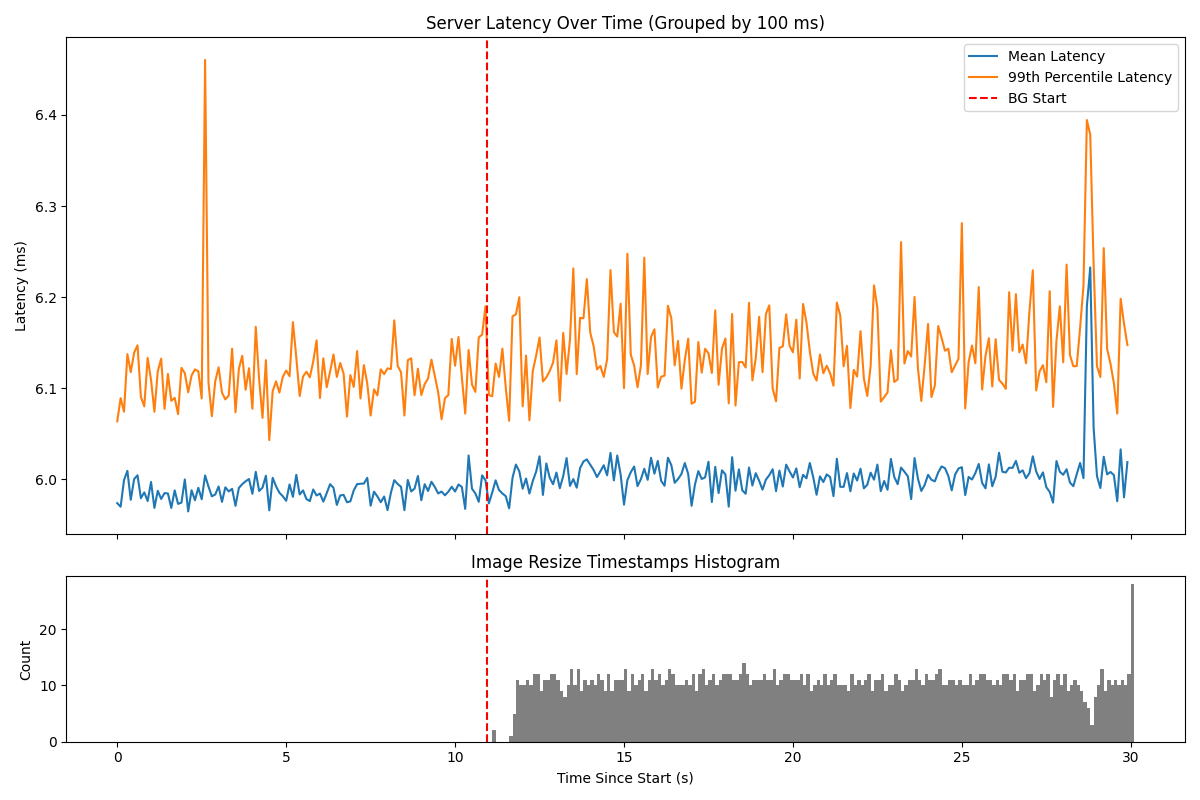
\includegraphics[width=\columnwidth]{graphs/srv-bg-rt-low.png}
        \caption{Low load}\label{fig:srv-bg-rt-low}
        \vspace{12pt}
    \end{subfigure}
    \hspace{\fill}
    \begin{subfigure}[t]{\columnwidth}
        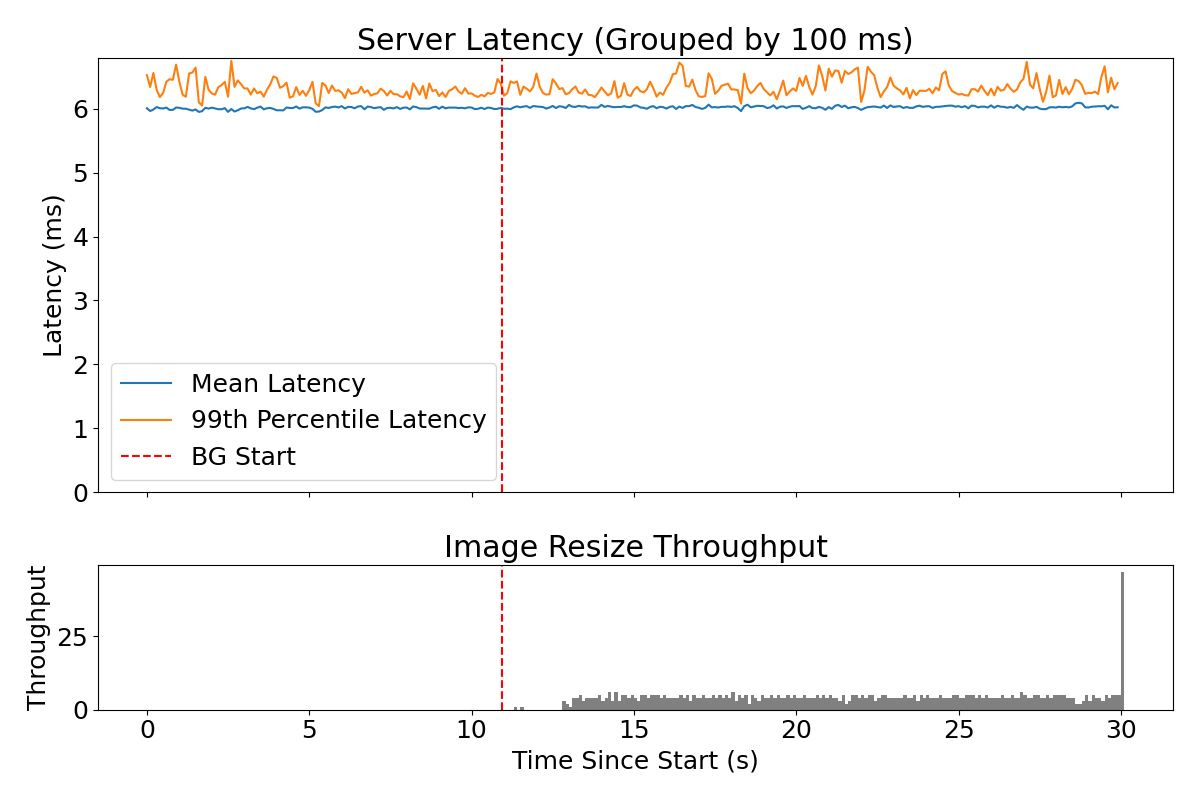
\includegraphics[width=\columnwidth]{graphs/srv-bg-rt-high.png}
        \caption{High load}\label{fig:srv-bg-rt-high}
    \end{subfigure}
    \vspace{4pt}
    \caption{Results of the same experiment as in \autoref{fig:srv-bg-unedited}
    and \autoref{fig:srv-bg-schedbe}, with LC running as a real time
    process}\label{fig:srv-bg-rt}
\end{figure}

\autoref{fig:srv-bg-rt} shows the result of running the same microbenchmark from
\autoref{fig:srv-bg-unedited}, but with the LC server running in the \rtclass{}
scheduling class. We can see that \rtclass{} is isolated from \normalclass{}
well: in both load settings the tail and average latency stays stable at
$\sim$6.0ms after starting the BE workload.

\subsection{Linux scheduling classes are not suited to enforce LC service
reservations}\label{ss:approach:linux-classes-bad-fit}

This points to a possible alternative to using \cgroups{}: run LC in the real
time \rtclass{} scheduling class and BE in \normalclass{}.\footnote{The
\deadlineclass{} scheduling class is not a good fit, since it requires accurate
knowledge of a processes runtime (processing time per request) and period (when
requests come in)} However, we show that the schedulers within each priority are
not suited for microservices (\autoref{sss:approch:linux:policies}), and that
Linux method of avoiding starvation is unfitting
(\autoref{sss:approach:linux:starve-throttle}).

\subsubsection{Real time schedulers are unsuitable for microservice
workloads}\label{sss:approch:linux:policies}

Running a microservice in \rtclass{} is an untenable way of isolating LC from BE
because of \rtclass{}'s intra-priority schedulers. Our goal is to honor the
reservations LC services make, they should not have to use different scheduling
mechanisms to be able to get that. \hmng{a little clumsy} \rtclass{} has two
different scheduling policies: \schedfifo{} and \schedrr{}. Both have 99
priorities between which they enforce strict priority; within priorities they
differ in the policy they enforce.

\schedfifo{} uses first-in-first-out run-to-completion scheduling. This means
that wihin each class, the process to run next will be the one that woke up
first, and it will run until it blocks or exits. When a blocked thread becomes
runnable again, that is counted as a wakeup and it will be put on the back of
the queue. This is known to have a failure mode of head-of-line (HoL) blocking
under varied request processing times, where long-running requests monopolize
the CPU while short requests wait in the queue.

\schedrr{} addresses this concern by running a round-robin scheduler that will
ensure Processor Sharing within priorities. However, \schedrr{} has no way way
of enforcing unequal splits, every process just gets the same scheduling quantum
and then gets put at the end of that priority's queue. Unequal splits is
precisely what weights are good at, and why they are used for LC services today.

\subsubsection{Linux throttles \rtclass{} processes under high load
}\label{sss:approach:linux:starve-throttle}

Schedulers running priority scheduling have to contend with the possibility of
starvation. Starvation can have many negative effects: it can cause deadlocks if
a low and high priority process share a lock (either in user-space or in
kernel-space), TCP connections can die while the process is being starved, and
it can miss interrupts like timers or completed i/o requests.

To avoid these, Linux chooses to carefully ensure that no process is ever
starved by throttling high class processes with high load. Linux has two
different safe guards that enforce that no process is ever starved. One is that
\rtclass{} is as a scheduling class rate-limited: there are tuneable parameters
\texttt{sched\_rt\_runtime} and \texttt{sched\_rt\_period}, that together define
a rate limit for the \rtclass{} as a whole. The other safegaurd is that, even
when set to be equal (ie \rtclass{} gets the full runtime each period if it
wants), the \normalclass{} scheduling class also has a so-called
\textit{deadline server}, which ensures it gets a small amount of time. The
deadline server is a `process' is in the \deadlineclass{} scheduling class with
a small amount of runtime per period, then when chosen will pass control on to
the \normalclass{} scheduler~\cite{lkml-deadline-srv}.

The throttling Linux chooses to do interferes with the goal of honoring
reservations, because it throttles the LC experiencing high load, which is
precisly when it needs its full reservation  most.


\begin{figure}[t]
    \centering
    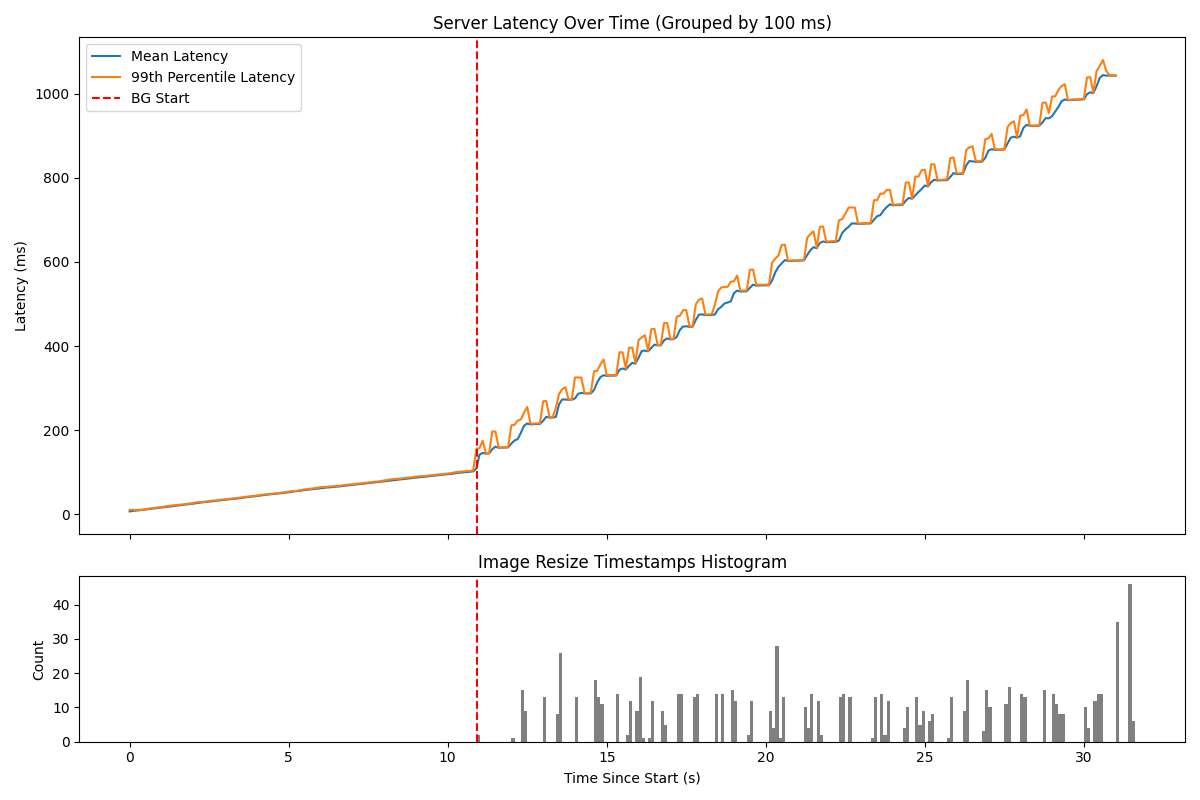
\includegraphics[width=\columnwidth]{graphs/overload-rt.png}
    \caption{LC in real time, throttling}\label{fig:overload-rt}
\end{figure}



Doing so impacts the performance of processes in the \rtclass{} at high load. We
can see this happen when we run the same microbenchmark experiment at a much
higher baseline utilization ($\sim$ 100\%). The results are in
\autoref{fig:overload-rt}. We see spikes begin to appear after starting the BE
task, as the \rtclass{} server gets throttled in favor of running the BE tasks;
we see parallel spikes in the BE's throughput in the bottom graph. Notice also
the increase of the slope of response times after starting the background tasks.

We conclude that Linux's mechanism of scheduling classes can isolate workloads
effectively, but that existing scheduling classes use algorithms that are not a
good fit for modern workloads, and that the isolation does not enforce
reservations because it throttles high priority class processes under high load.
